\documentclass[11pt,a4paper]{article}

\usepackage[utf8]{inputenc} 
\usepackage[T1]{fontenc} 
\usepackage{lmodern}
\usepackage[margin=2cm]{geometry}
\usepackage[german]{babel}
\usepackage{array}
\setlength{\parindent}{0pt}
\setlength{\parskip}{1ex plus 0.5ex minus 0.5ex}

\usepackage{amsmath} 
\usepackage{graphicx} 
\usepackage{booktabs}
\usepackage[colorlinks]{hyperref}
\usepackage{nicefrac}
\usepackage{gensymb}
\usepackage[usenames,dvipsnames,svgnames,table]{xcolor}
\usepackage{multirow}
\usepackage{tikz}
\usepackage[section]{placeins}

\hbadness=99999

\newcommand{\refpy}[1]{Siehe Anhang: \textit{Rechnungen in Python} (\texttt{{\color{incolor}In [{\color{incolor}#1}]}})}
\newcommand\dif{\mathop{}\!\mathrm{d}}
\newcommand{\halftime}[4]{\begin{figure}[h]
\begin{minipage}{.#1\textwidth}#3\end{minipage}\begin{minipage}{.#2\textwidth}
\centering
#4\end{minipage}
\end{figure}}
\renewcommand{\vec}{\boldsymbol}

\usepackage{etoolbox}

\makeatletter
\patchcmd{\@classz}
  {\CT@row@color}
  {\oldCT@column@color}
  {}
  {}
\patchcmd{\@classz}
  {\CT@column@color}
  {\CT@row@color}
  {}
  {}
\patchcmd{\@classz}
  {\oldCT@column@color}
  {\CT@column@color}
  {}
  {}
\makeatother

\newcommand{\rpm}{\raisebox{.2ex}{$\scriptstyle\pm$}}

\begin{document}

{
\centering 
\large 
Physiklabor für Anf\"anger*innen \\
Ferienpraktikum im Sommersemester 2018 \\[4mm]
\textbf{\LARGE 
Versuch 17: Trägheitsmomente/Steinerscher Satz
} \\[3mm]
(durchgef\"uhrt am 17.09.2018 bei Adrian Hauber)\\
Gruppe 14: Andréz Gockel, Patrick M\"unnich\\ 
\today \\[10mm]
}

\tableofcontents
\vspace{22pt}
\listoffigures
\vspace{22pt}
\listoftables
\pagebreak



\section{Ziel des Versuchs}

Dieser Versuch hat zwei Teile. Im ersten Teil wird mit Hilfe von einer hergeleiteten Formel (\ref{}), die den Trägheitsmoment mit der Periodendauer in Zusammenhang bringt das Trägheitsmoment eines ausgedehnten starren Körper berechnet. Dieses wird verglichen mit dem experimentell bestimmten Wert. Das Trägheitsmoment wird bestimmt von einer zylindrische Stange, die nicht im Schwerpunkt aufgehängt wird und die per hand in Schwingung versetzt wird, in dem die Schwingungsdauer gemessen wird und den Wert mit der hergeleiteten Formel berechnet wird. In dem zweiten Teil wird von einem Drehpendel den Zusammenhang von der Schwingungsdauer und dem Abstand von einer Zusatzmasse zum Mittelpunkt verwendet, um hiermit den Steinerschen Satz experimentell zu verifizieren. 

\section{Teil 1 - Trägheitsmomente}
\subsection{Herleitung der Schwingungsgelichung}

Der unterschied von einem mathematischen Pendel und einem physikalischen Pendels ist dass, es sich nicht um eine punktförmige Masse handelt sondern den Schwerpunkt von einem starren Körper wo das Trägheitsmoment berücksichtigt werden muss. Mit der rücktreibenden Kraft $F_r = mg\sin\varphi$ und den Abstand von Aufhängepunkt zu Schwerpunkt $d$ können wir das Drehmoment ausdrücken als:
$$\vec{M} = \vec{F_r} \times \vec{d} = dm\vec{g}\sin(\varphi)$$
mit der klein Winkel Näherung: $\sin\varphi \approx \varphi$:
$$\vec{M} = dm\vec{g}\varphi$$
Dies wird gleichgesetzt mit:
$$\vec{M} = \vec{\dot L} = - I \cdot \vec{\dot\omega} = - I \cdot \ddot \varphi$$
$$\Rightarrow - I \cdot \ddot \varphi = dm\vec{g}\varphi \quad \Rightarrow \ddot \varphi = - \bigg(\underbrace{\frac{dm\vec{g}}{I}}_{\omega^2}\bigg)\varphi \quad \Rightarrow \ddot \varphi = - \omega^2 \varphi$$
Mit $T = 2\pi \frac{1}{\vec{\omega}}$ bekommt man: $T = 2\pi \sqrt{\frac{I}{dm\vec{g}}}$.

Zunächst wird das Trägheitsmoment eines starren Körpers, in diesem fall einen Stab (Vollzylinder) berechnet. Allgemein für das Trägheitsmoment bezüglich der Drehachse gilt:
$$I = \int \vec{r}^2 \dif m$$
mit $m = \rho V$ und angenommen der Zylinder ist homogen bekommt man: $\displaystyle{I_{\textrm{stab}} = \rho \int_V \vec{r}^2 \dif V}$

in Zylinderkoordinaten: $\vec{r}^2 = $
$$I = \rho \int\displaylimits_{0}^{2\pi} \int\displaylimits_{0}^{l}\int\displaylimits_{0}^{r}\dif\phi \dif z \dif r$$ 
wobei 
\subsection{Aufbau}

\halftime{5}{5}{Ein zylindrischer Stab der an einem Stativ gehängt werden kann. Zusätzlich wird benötigt ein Bandmass, Messschieber und eine Stoppuhr für die Messungen. }{
\centering
\fbox{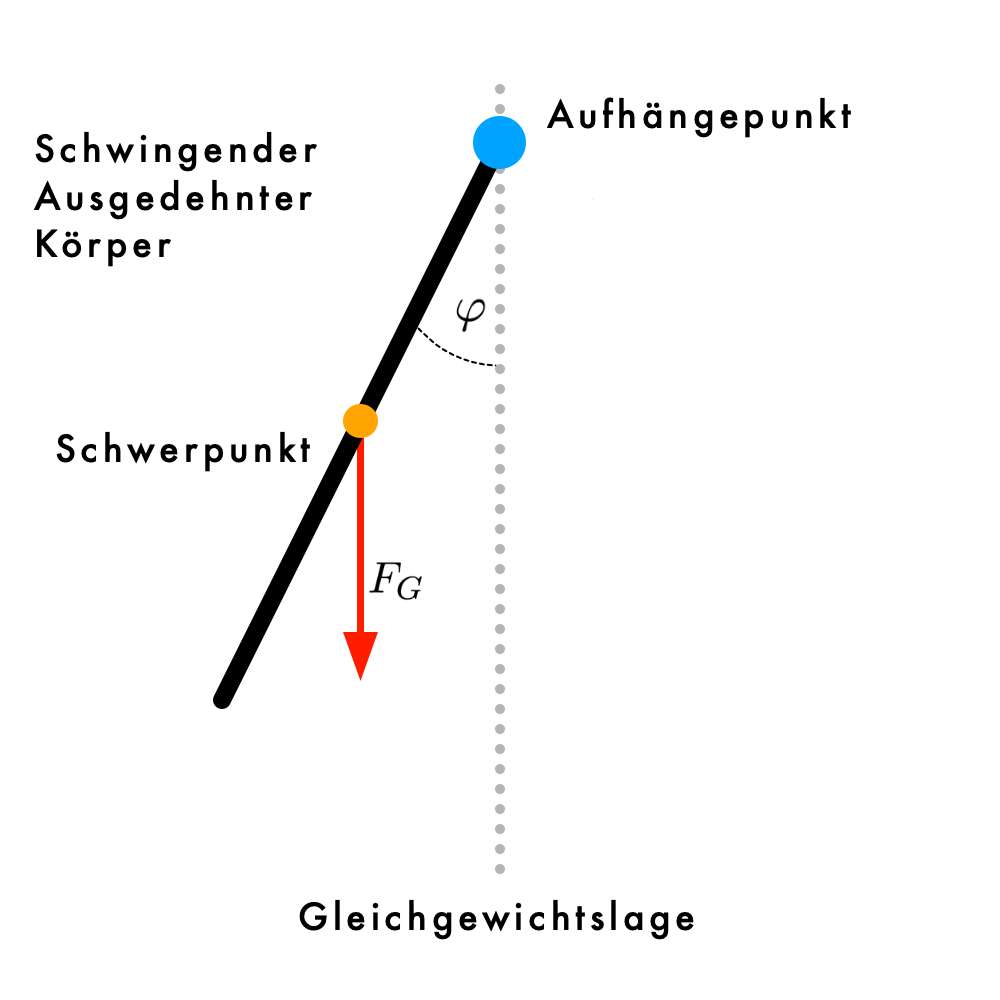
\includegraphics[width=0.5\textwidth]{Spend}}
   \renewcommand\thefigure{B1}
\caption{Versuchsaufbau 1}
\label{JS1}
}

\FloatBarrier
\subsection{Durchführung}

Zuerst wurde die Länge des Stabes mittels Bandmass gemessen. Zunächst wurde mittels Messschieber der Durchmesser des Stabes gemißt. Dann wurde der Stab and das Stativ gehängt und per hand zum pendeln gebracht. Es wurde mit der Stoppuhr 30 mal eine Periode zeitlich gemessen. Danach wurde ein mal 30 Perioden gemißt, um zu schauen welches verfahren ein kleineren Fehler hat. Dies ergab sich als das zweite verfahren. 

\subsubsection{Auswertung}

\begin{table}[ht]
\caption{Relevante Werte (Teil 2)}
$$
\begin{array}{lc}
	\multicolumn{1}{l}{\textrm{Zu Bestimmende Werte}} \\
	\toprule 
	\textrm{Stablänge} & l = 95.6(3)\,\textrm{cm} \\
	\textrm{Radius} & r = 5.0(2)\,\textrm{mm} \\
	\bottomrule 
\end{array}
$$
\end{table}


\pagebreak

\section{Teil 2 - Steinersche Satz}

\subsection{Aufbau}

\halftime{5}{5}{Zu diesem Versuch wurde ein Drehpendel verwendet der aus einer Zusatzmasse, Drehtisch und einer Spiralfeder besteht. Die Zusatzmasse kann in verschiedenen abständen von dem Mittelpunkt befestigt werden. Für die Messungen wurde eine Stoppuhr, und einen Messschieber verwendet.}{
\centering
\fbox{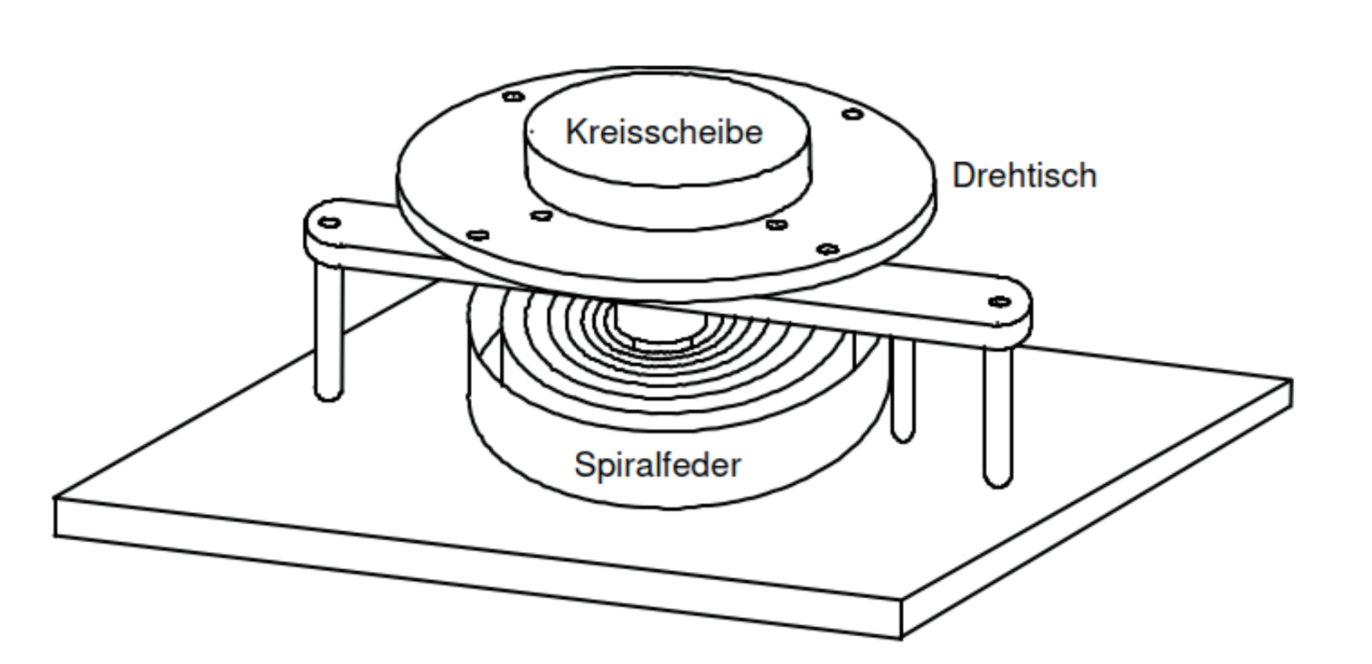
\includegraphics[width=0.7\textwidth]{Drehp}}
   \renewcommand\thefigure{B2}
\caption[Versuchsaufbau 2]{Versuchsaufbau 2 \cite{Anleitung}}
\label{B2}
}

\subsubsection{Durführung}

Es wurden Breite und Durchmesser der Zusatzmasse mit dem Messschieber gemißt. (Die Masse wurde schon vorher gemessen und auf oben drauf Geschrieben.) Zunächst wurde die Zeit für 30 Perioden ohne Zusatzmasse gemessen. Zunächst wurde die Masse in den Mittelpunkt gesetzt und Drehtisch wurde von hand soweit aus gelenkt damit 30 Perioden zeitlich gemessen werden konnten. Dies wurde wiederholt für 10 Perioden. Anschliessend wurde die Masse mit einem abstand von 15\,mm versetzt und wieder jeweils 30 und 10 Perioden gemessen. Dies wurde wiederholt für vier weitere abstände. 

\subsection{Auswertung}

\begin{table}[ht]
\caption{Relevante Werte (Teil 2)}
$$
\begin{array}{ll}
	\multicolumn{1}{l}{\textrm{Zu Bestimmende Werte}} \\
	\toprule 
	\textrm{Zusatzmasse} & m = 1.109(5)\,\textrm{kg} \\
	\textrm{Durchmesser} & d = 118.9(1)\,\textrm{mm} \\
	\textrm{Breite} & h = 12.9(1)\,\textrm{mm} \\
	\bottomrule \\
	\multicolumn{2}{l}{\textrm{Bekannte Werte}} \\
	\toprule
	\textrm{Abstände} & a = 15.0\,\textrm{mm}\\
	\bottomrule 
\end{array}
$$
\end{table}




\vfill

\begin{thebibliography}{9}
 \bibitem{Uncertainties}''Correlations between variables are automatically handled, which sets this module apart from many existing error propagation codes.'' - https://pythonhosted.org/uncertainties/
 \bibitem{Anleitung} Physikalisches Institut der Albert-Ludwigs-Universität Freiburg (Hrsg.) (08/2018): Versuchsanleitungen zum Physiklabor für Anfänger*innen, Teil 1, Ferienpraktikum im Sommersemester 2018.
 \end{thebibliography}
 
%Systematische und statistische Fehler.

\pagebreak


\section{Anhang}

\begin{table}[h]
\caption{Messwerte (Teil 2)}
$$
\begin{array}{ccc}	
	\toprule 
	\textrm{Abstand/mm} & \textrm{10 Perioden/s} & \textrm{30 Perioden/s}\\
	\midrule
	\multicolumn{1}{l}{\textrm{Ohne Zusatzmasse}} & 18.1 & 54.6\\
	\phantom{zz.}0 & 20.6 & 60.3\\
	15.0 & 20.8 & 63.0\\
	30.0 & 21.8 & 63.2\\
	45.0 & 22.9 & 68.9\\
	60.0 & 24.9 & 72.0\\
	\bottomrule 
\end{array}
$$
\end{table}



\end{document}